\documentclass[12pt,a4paper]{article}

% ============================================================
% PACKAGES
% ============================================================
\usepackage[utf8]{inputenc}
\usepackage[T1]{fontenc}
\usepackage[french]{babel}
\usepackage{geometry}
\usepackage{graphicx}
\graphicspath{{images/}}
\usepackage{xcolor}
\usepackage{listings}
\usepackage{booktabs}
\usepackage{array}
\usepackage{hyperref}
\usepackage{fancyhdr}
\usepackage{titlesec}
\usepackage{enumitem}
\usepackage{mdframed}
\usepackage{tikz}
\usepackage{float}
\usepackage[table]{xcolor}

% ============================================================
% MISE EN PAGE
% ============================================================
\geometry{
  top=2.5cm,
  bottom=2.5cm,
  left=2.5cm,
  right=2.5cm
}

% ============================================================
% COULEURS
% ============================================================
\definecolor{primary}{RGB}{30, 100, 180}
\definecolor{secondary}{RGB}{240, 245, 255}
\definecolor{codebg}{RGB}{245, 245, 245}
\definecolor{codeframe}{RGB}{200, 200, 200}
\definecolor{success}{RGB}{39, 174, 96}
\definecolor{warning}{RGB}{230, 126, 34}
\definecolor{darkgray}{RGB}{60, 60, 60}

% ============================================================
% EN-TETE ET PIED DE PAGE
% ============================================================
\pagestyle{fancy}
\fancyhf{}
\fancyhead[L]{\small\textcolor{primary}{\textbf{Projet M1 GIL -- Gestion de Flotte}}}
\fancyhead[R]{\small\textcolor{darkgray}{Universite de Rouen | 2025--2026}}
\fancyfoot[C]{\thepage}
\renewcommand{\headrulewidth}{0.4pt}

% ============================================================
% STYLE DES TITRES
% ============================================================
\titleformat{\section}
  {\Large\bfseries\color{primary}}
  {\thesection.}{0.8em}{}[\titlerule]

\titleformat{\subsection}
  {\large\bfseries\color{darkgray}}
  {\thesubsection.}{0.6em}{}

\titleformat{\subsubsection}
  {\normalsize\bfseries\color{darkgray}}
  {\thesubsubsection.}{0.5em}{}

% ============================================================
% STYLE DU CODE
% ============================================================
\lstset{
  backgroundcolor=\color{codebg},
  frame=single,
  rulecolor=\color{codeframe},
  basicstyle=\ttfamily\small,
  keywordstyle=\color{primary}\bfseries,
  commentstyle=\color{gray}\itshape,
  stringstyle=\color{success},
  breaklines=true,
  showstringspaces=false,
  numbers=left,
  numberstyle=\tiny\color{gray},
  numbersep=8pt,
  tabsize=2,
  captionpos=b
}

% ============================================================
% BOITE INFO
% ============================================================
\newmdenv[
  backgroundcolor=secondary,
  linecolor=primary,
  linewidth=1.5pt,
  leftline=true,
  rightline=false,
  topline=false,
  bottomline=false,
  innerleftmargin=10pt,
  innerrightmargin=10pt,
  innertopmargin=8pt,
  innerbottommargin=8pt
]{infobox}

% ============================================================
% COMMANDE PLACEHOLDER SCREENSHOT
% ============================================================
\newcommand{\screenshot}[2]{%
  \begin{figure}[H]
    \centering
    \begin{tikzpicture}
      \draw[dashed, color=gray, line width=1pt]
        (0,0) rectangle (14cm, 5cm);
      \node[color=gray] at (7cm, 2.7cm)
        {\large\textbf{[ CAPTURE D'ECRAN ]}};
      \node[color=gray] at (7cm, 2.1cm)
        {\normalsize #1};
    \end{tikzpicture}
    \caption{#2}
  \end{figure}
}

% ============================================================
% DOCUMENT
% ============================================================
\begin{document}

% ------------------------------------------------------------
% PAGE DE TITRE
% ------------------------------------------------------------
\begin{titlepage}
  \centering
  \vspace*{1cm}

  {\Large\textbf{Universite de Rouen Normandie}\\[0.3cm]
  \large Master 1 -- Genie Informatique et Logiciel}

  \vspace{1.5cm}
  \rule{\linewidth}{0.5mm}\\[0.4cm]

  {\Huge\bfseries\color{primary} Projet Gestion de Flotte de vehicules\\[0.3cm]}
  {\LARGE\bfseries Rapport de Semaine 3}\\[0.3cm]
  {\large\color{darkgray} Microservice Véhicules}

  \rule{\linewidth}{0.5mm}\\[1.5cm]

  \begin{minipage}{0.45\textwidth}
    \begin{flushleft}
      \textbf{Etudiant :}\\
      Ahcene Amouchas \\
      Florian Pepin \\[0.5cm]
      \textbf{Encadrants :}\\
      Lydia \& Luc
    \end{flushleft}
  \end{minipage}
  \hfill
  \begin{minipage}{0.45\textwidth}
    \begin{flushright}
      \textbf{Annee universitaire :}\\
      2025 -- 2026\\[0.5cm]
      \textbf{Semaine :}\\
      3 / 7
    \end{flushright}
  \end{minipage}

  \vfill
  {\large\today}
\end{titlepage}

% ------------------------------------------------------------
% TABLE DES MATIERES
% ------------------------------------------------------------
\tableofcontents
\newpage

% ------------------------------------------------------------
% INTRODUCTION
% ------------------------------------------------------------
\section{Introduction et objectifs de la semaine}

\begin{infobox}
\textbf{Objectif de la semaine 3 :} Développer le premier microservice fonctionnel du service véhicules en respectant les bonnes pratiques de
qualité logicielle : tests, couverture de code, et observabilité intégrée dès le départ.
\end{infobox}

\vspace{0.5cm}

La semaine 3 du projet marque le passage de l'infrastructure au développement métier.
L'équipe s'est concentrée sur la conception et l'implémentation du service de véhicules qui est le socle du système de gestion de flotte.

Les grandes étapes réalisées sont les suivantes :

\begin{enumerate}[leftmargin=*, label=\textbf{\arabic*.}]
  \item Développement de l'\textbf{API REST} complète (CRUD véhicules avec validation des données)
  \item Intégration d'\textbf{Apache Kafka} en tant que producer/consumer pour les événements métier
  \item Création des \textbf{résolveurs GraphQL} pour l'agrégation future entre services
  \item \textbf{Tests unitaires (>80\% couverture) et d’intégration}
  \item Instrumentation du service avec le \textbf{SDK OpenTelemetry} (traces, métriques, logs structurés)
\end{enumerate}

% ============================================================
% SECTION : MISE EN ŒUVRE DU CRUD VÉHICULES
% ============================================================
\newpage
\section{Mise en œuvre du microservice de gestion des véhicules}

L'une des briques centrales du système est le microservice de gestion de la flotte. Cette section détaille l'implémentation du CRUD (Create, Read, Update, Delete) pour l'entité \texttt{Vehicle}, en suivant une architecture en couches propre à Spring Boot.

\subsection{Modèle de données et Soft Delete}
L'entité \texttt{Vehicle} est conçue pour être persistée dans une base de données PostgreSQL. Une particularité de l'implémentation est l'usage du \textbf{Soft Delete} : au lieu de supprimer physiquement une ligne, nous renseignons un champ \texttt{deletedAt}.

\begin{lstlisting}[language=Java, caption=Entité Vehicle avec énumérations PostgreSQL]
@Entity
@Table(name = "vehicles")
public class Vehicle {
    @Id
    @GeneratedValue(strategy = GenerationType.UUID)
    private UUID id;

    @Column(name = "plate_number", nullable = false, unique = true)
    private String plateNumber;

    @Enumerated(EnumType.STRING)
    @JdbcTypeCode(SqlTypes.NAMED_ENUM)
    private VehicleStatus status = VehicleStatus.available;

    private OffsetDateTime deletedAt; // Pour le Soft Delete
}
\end{lstlisting}

\subsection{Couche Accès aux Données (Repository)}
Pour supporter le mécanisme de suppression logique, le \texttt{VehicleRepository} définit des requêtes JPQL spécifiques qui filtrent les enregistrements dont la date de suppression est nulle.

\begin{lstlisting}[language=Java, caption=Requêtes personnalisées pour le Soft Delete]
@Repository
public interface VehicleRepository extends JpaRepository<Vehicle, UUID> {
    @Query("SELECT v FROM Vehicle v WHERE v.deletedAt IS NULL")
    List<Vehicle> findAllActive();

    @Query("SELECT v FROM Vehicle v WHERE v.id = :id AND v.deletedAt IS NULL")
    Optional<Vehicle> findByIdActive(UUID id);
}
\end{lstlisting}

\subsection{Logique Métier et DTOs}
L'exposition des données ne se fait pas directement via l'entité, mais par des \textbf{Java Records} (DTOs), garantissant l'immutabilité et la validation des entrées.

\begin{itemize}
    \item \textbf{Validation} : Utilisation de \texttt{@NotBlank} et \texttt{@Min} dans \texttt{VehicleInput} pour valider les payloads.
    \item \textbf{Mapping} : Le service transforme les entités en \texttt{VehicleResponse} avant de les retourner au contrôleur.
\end{itemize}

\subsection{Contrôleur REST}
Le \texttt{VehicleController} expose les points de terminaison nécessaires à la gestion de la flotte. Voici le récapitulatif des routes implémentées :

\begin{center}
\begin{tabular}{|l|l|l|}
  \hline
  \rowcolor{primary!10}
  \textbf{Méthode} & \textbf{Point de terminaison} & \textbf{Action} \\
  \hline
  GET    & \texttt{/vehicles}          & Liste tous les véhicules actifs \\
  GET    & \texttt{/vehicles/\{id\}}   & Détails d'un véhicule spécifique \\
  POST   & \texttt{/vehicles}          & Création d'un véhicule (Validation active) \\
  PUT    & \texttt{/vehicles/\{id\}}   & Mise à jour des informations \\
  PATCH  & \texttt{/vehicles/\{id\}/status} & Modification rapide du statut \\
  DELETE & \texttt{/vehicles/\{id\}}   & Suppression logique (Soft Delete) \\
  \hline
\end{tabular}
\end{center}

\begin{lstlisting}[language=Java, caption=Extrait du contrôleur pour la suppression logique]
@DeleteMapping("/{id}")
@ResponseStatus(HttpStatus.NO_CONTENT)
public void deleteVehicle(@PathVariable UUID id) {
    service.deleteVehicle(id);
}
\end{lstlisting}

Cette structure assure que les données critiques restent en base pour la traçabilité (historique des livraisons) tout en étant invisibles pour les opérations courantes de l'application.

\newpage

% ------------------------------------------------------------
% TESTS AVEC POSTMAN
% ------------------------------------------------------------
\section{Tests de l'API REST avec Postman}

\begin{infobox}
\textbf{Objectif :} Valider le bon fonctionnement de l'ensemble des endpoints du service
Véhicules via des tests manuels réalisés avec \textbf{Postman}, couvrant les opérations
CRUD ainsi que la gestion des assignations.
\end{infobox}

\vspace{0.5cm}

L'ensemble des routes exposées par le service Véhicules ont été testées manuellement
à l'aide de Postman. Les tests couvrent les deux ressources principales : les
\textbf{véhicules} et leurs \textbf{assignations}. Chaque requête a retourné le code
HTTP attendu, confirmant la conformité de l'API aux standards REST.

\subsection{CRUD Véhicules}

\subsubsection*{POST /vehicles — Ajout d'un véhicule}

La création d'un véhicule s'effectue via une requête \texttt{POST} sur
\texttt{/vehicles}. Le corps de la requête contient les informations du véhicule
(\texttt{plateNumber}, \texttt{brand}, \texttt{model}, \texttt{fuelType},
\texttt{mileageKm}, \texttt{vin}, \texttt{payloadCapacityKg}, \texttt{cargoVolumeM3}).
Le service retourne un \textbf{201 Created} avec l'objet créé, incluant l'UUID généré
automatiquement et le statut par défaut \texttt{available}.

\begin{figure}[H]
  \centering
  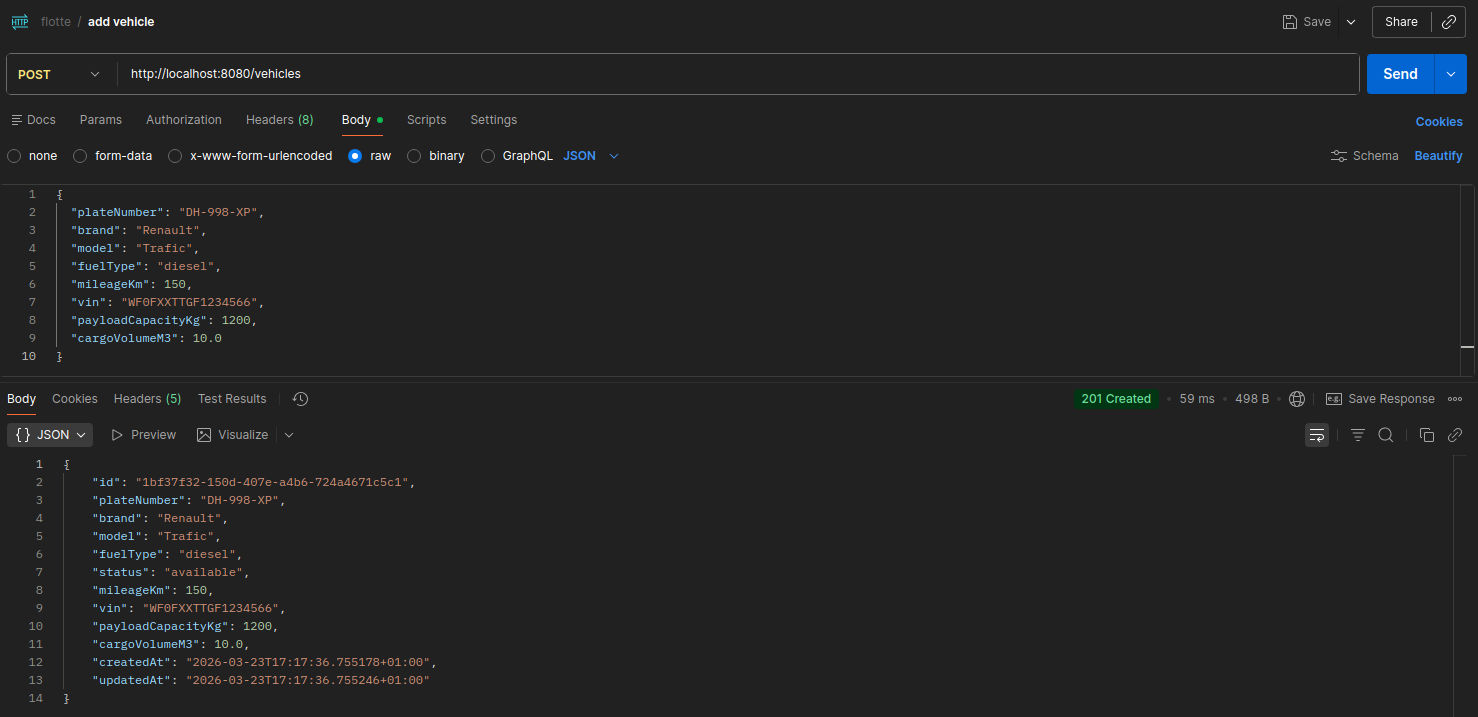
\includegraphics[width=\linewidth]{./images/postman-8.png}
  \caption{POST /vehicles — Création d'un véhicule (201 Created)}
\end{figure}

\begin{figure}[H]
  \centering
  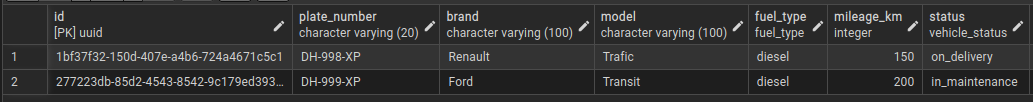
\includegraphics[width=\linewidth]{./images/postman-9.png}
  \caption{POST /vehicles — Détails}
\end{figure}

\subsubsection*{GET /vehicles — Liste de tous les véhicules}

Une requête \texttt{GET} sur \texttt{/vehicles} retourne la liste des véhicules
non supprimés. Le mécanisme de \textbf{soft delete} est ici mis en évidence : seuls
les véhicules actifs sont retournés, même si la base de données en contient davantage.
Le serveur répond avec un \textbf{200 OK}.

\begin{figure}[H]
  \centering
  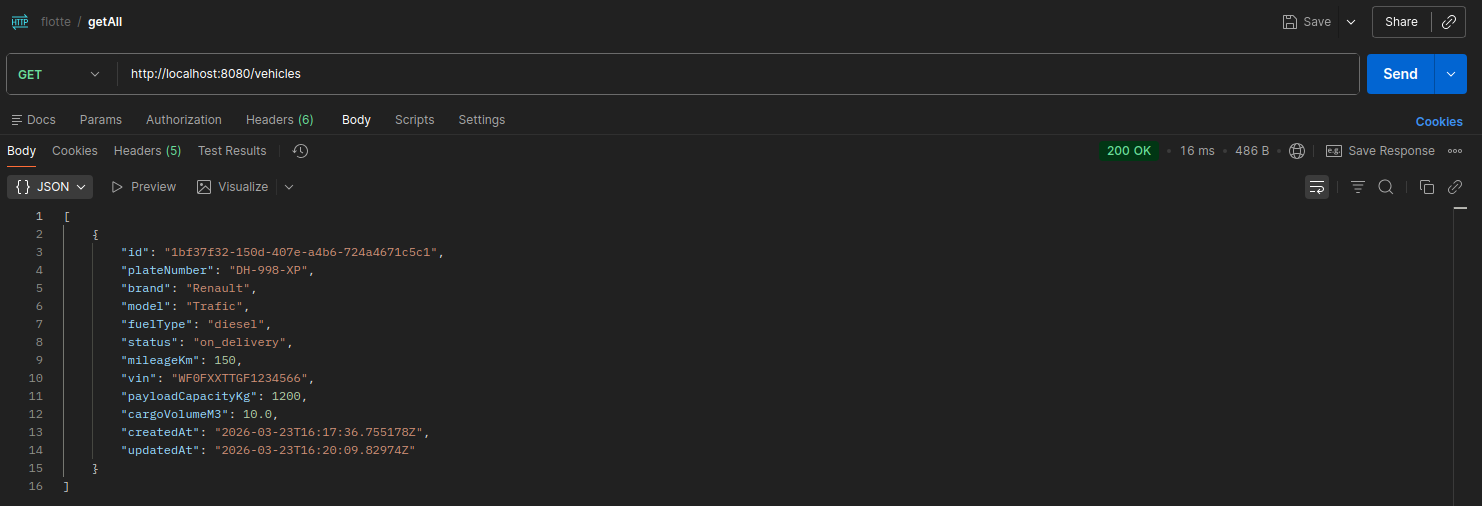
\includegraphics[width=\linewidth]{./images/postman-7.png}
  \caption{GET /vehicles — Récupération de la liste des véhicules (200 OK)}
\end{figure}

\subsubsection*{GET /vehicles/:id — Récupération par identifiant}

La récupération d'un véhicule précis s'effectue en passant son UUID en paramètre
de chemin. Le service retourne un \textbf{200 OK} avec l'intégralité des champs
du véhicule correspondant.

\begin{figure}[H]
  \centering
  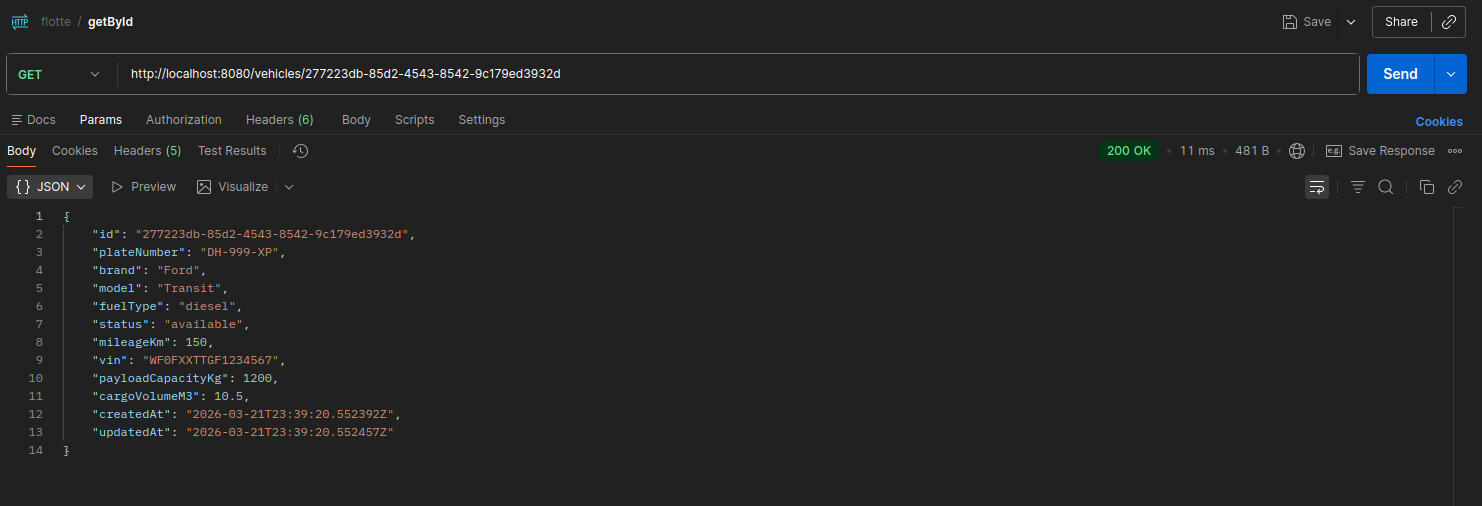
\includegraphics[width=\linewidth]{./images/postman-6.png}
  \caption{GET /vehicles/:id — Récupération d'un véhicule par UUID (200 OK)}
\end{figure}

\subsubsection*{PUT /vehicles/:id — Mise à jour complète}

La mise à jour d'un véhicule via \texttt{PUT} remplace les champs modifiables
(\texttt{mileageKm}, \texttt{brand}, \texttt{model}, etc.). Le service retourne
un \textbf{200 OK} avec les données mises à jour et un \texttt{updatedAt} rafraîchi.

\begin{figure}[H]
  \centering
  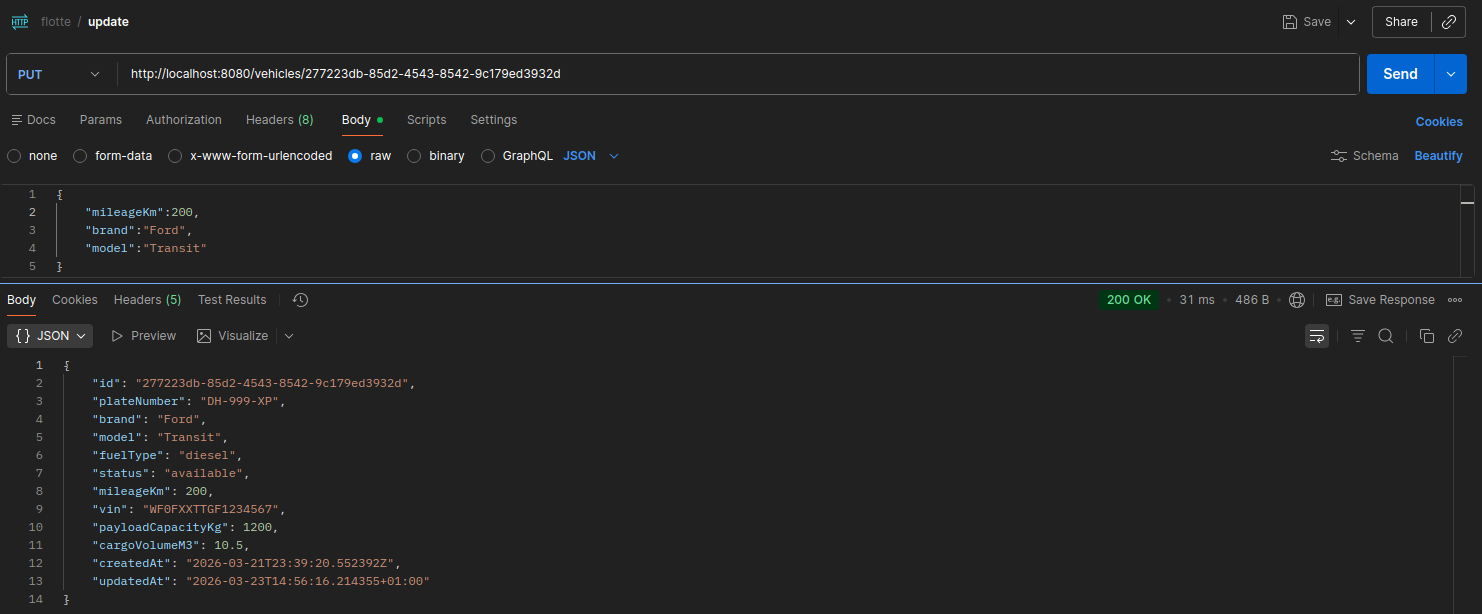
\includegraphics[width=\linewidth]{./images/postman-5.png}
  \caption{PUT /vehicles/:id — Mise à jour complète d'un véhicule (200 OK)}
\end{figure}

\newpage

\subsubsection*{PATCH /vehicles/:id/status — Mise à jour du statut}

Une route dédiée permet de modifier uniquement le statut d'un véhicule (ex.
\texttt{available}, \texttt{in\_maintenance}, \texttt{on\_delivery}). Cette approche
évite d'envoyer l'intégralité du corps pour un changement ponctuel. Le service
répond avec un \textbf{200 OK} et retourne le véhicule avec son nouveau statut.

\begin{figure}[H]
  \centering
  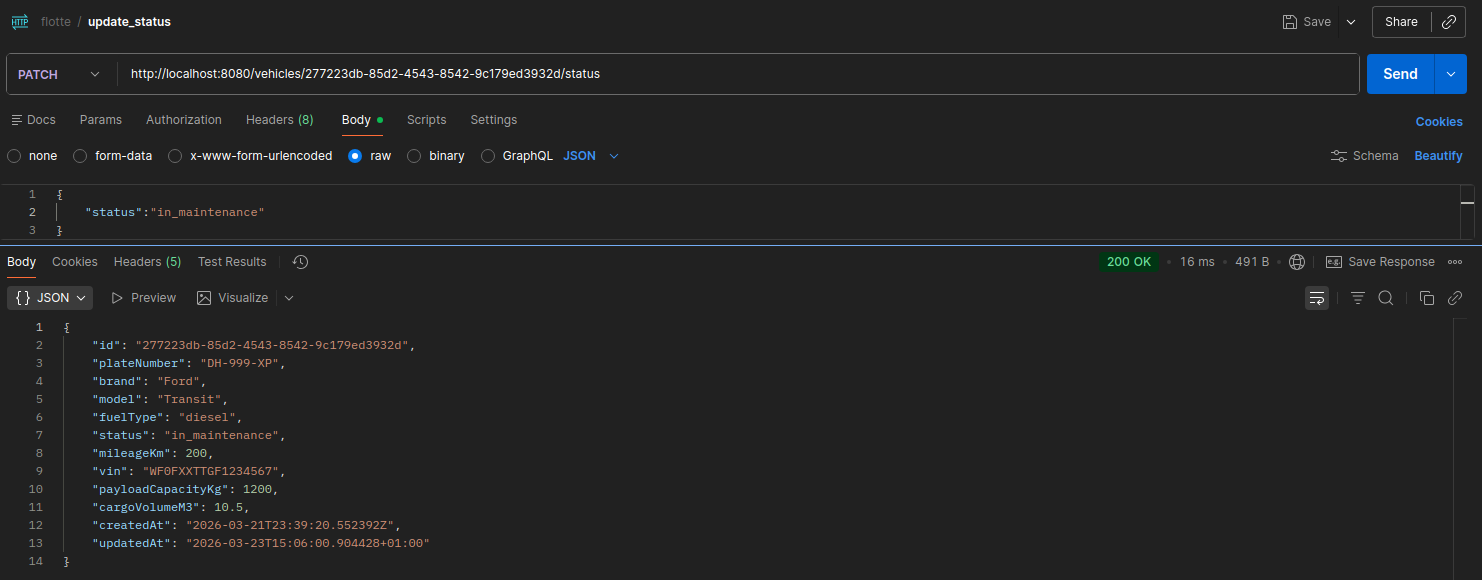
\includegraphics[width=\linewidth]{./images/postman-4.png}
  \caption{PATCH /vehicles/:id/status — Mise à jour du statut (200 OK)}
\end{figure}

\subsubsection*{DELETE /vehicles/:id — Suppression logique}

La suppression d'un véhicule est implémentée en \textbf{soft delete} : le véhicule
n'est pas physiquement retiré de la base de données mais marqué comme supprimé.
Le service retourne un \textbf{204 No Content}, et le véhicule disparaît des
résultats des requêtes \texttt{GET}. La base de données (visible via pgAdmin)
conserve bien les deux entrées, confirmant ce comportement.

\begin{figure}[H]
  \centering
  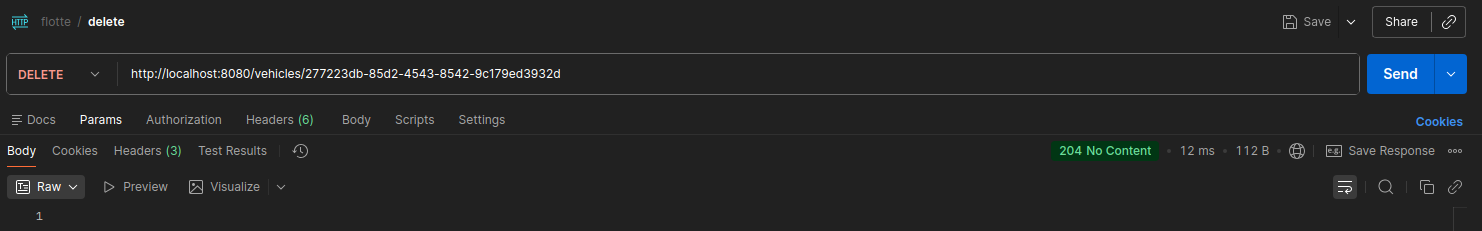
\includegraphics[width=\linewidth]{./images/postman-3.png}
  \caption{DELETE /vehicles/:id — Suppression logique (204 No Content)}
\end{figure}

\newpage

\subsection{Gestion des assignations}

\subsubsection*{POST /vehicles/:id/assignments — Ajout d'une assignation}

L'assignation d'un conducteur à un véhicule s'effectue via une requête \texttt{POST}
sur \texttt{/vehicles/:id/assignments}. Le corps contient le \texttt{driverId},
des \texttt{notes} optionnelles et le \texttt{createdBy}. Le service répond avec
un \textbf{201 Created} et retourne l'assignation créée avec sa date de début.

\begin{figure}[H]
  \centering
  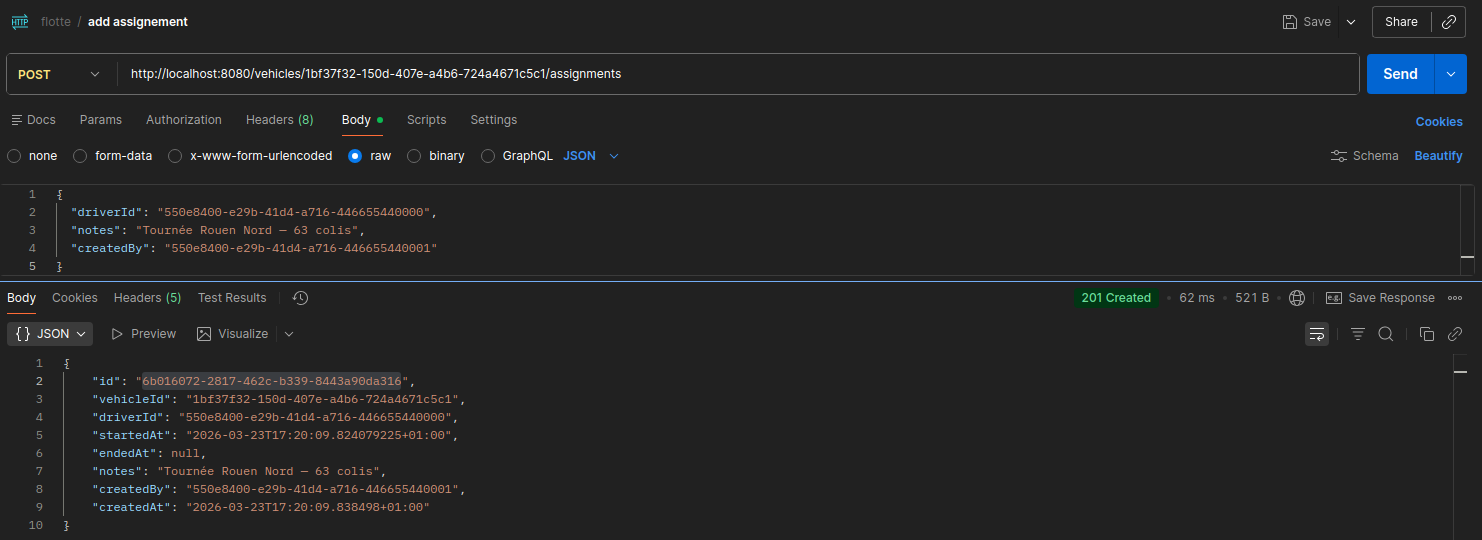
\includegraphics[width=\linewidth]{./images/postman-2.png}
  \caption{POST /vehicles/:id/assignments — Création d'une assignation (201 Created)}
\end{figure}

\subsubsection*{GET /vehicles/:id/assignments — Liste des assignations}

La récupération des assignations d'un véhicule retourne l'historique complet des
affectations de conducteurs. Le champ \texttt{endedAt} à \texttt{null} indique
une assignation en cours. Le service répond avec un \textbf{200 OK}.

\begin{figure}[H]
  \centering
  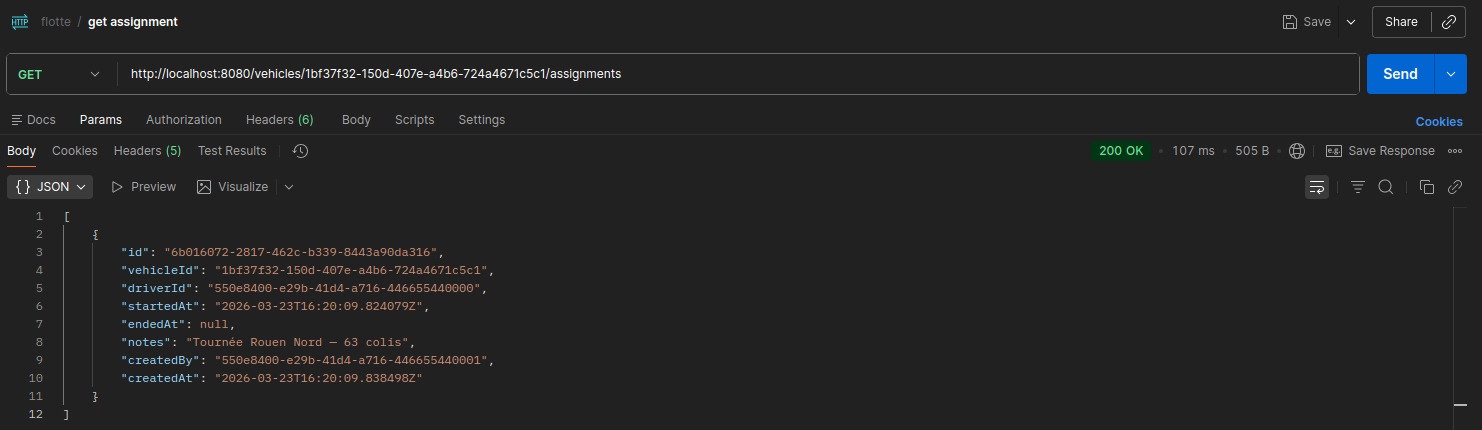
\includegraphics[width=\linewidth]{./images/postman-1.png}
  \caption{GET /vehicles/:id/assignments — Liste des assignations (200 OK)}
\end{figure}

\subsection{Bilan des tests}

\begin{center}
\begin{tabular}{|l|l|l|c|}
  \hline
  \textbf{Requête} & \textbf{Endpoint} & \textbf{Code attendu} & \textbf{Résultat} \\
  \hline
  POST   & /vehicles                       & 201 Created    & \textcolor{green!60!black}{\textbf{OK}} \\
  GET    & /vehicles                       & 200 OK         & \textcolor{green!60!black}{\textbf{OK}} \\
  GET    & /vehicles/:id                   & 200 OK         & \textcolor{green!60!black}{\textbf{OK}} \\
  PUT    & /vehicles/:id                   & 200 OK         & \textcolor{green!60!black}{\textbf{OK}} \\
  PATCH  & /vehicles/:id/status            & 200 OK         & \textcolor{green!60!black}{\textbf{OK}} \\
  DELETE & /vehicles/:id                   & 204 No Content & \textcolor{green!60!black}{\textbf{OK}} \\
  POST   & /vehicles/:id/assignments       & 201 Created    & \textcolor{green!60!black}{\textbf{OK}} \\
  GET    & /vehicles/:id/assignments       & 200 OK         & \textcolor{green!60!black}{\textbf{OK}} \\
  \hline
\end{tabular}
\end{center}

\vspace{0.3cm}
L'ensemble des 8 endpoints testés retournent les codes HTTP attendus. Le soft delete
est correctement implémenté et le filtrage des véhicules supprimés fonctionne comme
prévu.

% ------------------------------------------------------------
% IRESOLVEURS GRAPHQL
% ------------------------------------------------------------
\section{Résolveurs GraphQL}

\begin{infobox}
\textbf{Objectif :} Exposer les données du service Véhicules via une couche
\textbf{GraphQL} portée par l'API Gateway, en séparant clairement les résolveurs
fonctionnels des résolveurs non encore branchés aux microservices.
\end{infobox}

\vspace{0.5cm}

L'API Gateway agrège les résolveurs de l'ensemble des microservices en un schéma
GraphQL unifié. Pour la semaine 3, seuls les résolveurs liés au service Véhicules
sont pleinement opérationnels. Les autres (conducteurs, alertes, localisation,
maintenance) sont provisoirement remplacés par des \textbf{stubs} qui retournent
une erreur explicite, évitant tout comportement silencieux.

\subsection{Architecture des résolveurs}

Les résolveurs sont organisés en trois fichiers distincts :

\begin{itemize}
  \item \texttt{vehicleResolvers.ts}: résolveurs actifs, branchés sur le service Véhicules.
  \item \texttt{stubResolvers.ts}: résolveurs non encore implémentés, retournant une
        erreur \texttt{NOT\_IMPLEMENTED}.
  \item \texttt{index.ts}: point d'entrée fusionnant les deux via spread operator.
\end{itemize}

\vspace{0.3cm}
Le fichier \texttt{index.ts} assemble les résolveurs de façon non destructive :
les clés de \texttt{vehicleResolvers} écrasent celles des stubs pour les champs
déjà implémentés, ce qui permet d'enrichir progressivement le schéma semaine
après semaine sans modifier la structure d'agrégation.

\newpage

\subsection{Résolveurs Véhicules}

\subsubsection*{Queries}

Trois queries sont exposées et délèguent directement au contexte GraphQL
(\texttt{ctx.vehicle}) :

\begin{itemize}
  \item \texttt{vehicles}: liste des véhicules avec filtrage optionnel
        par statut (\texttt{status}, \texttt{limit}, \texttt{offset} avec valeurs
        par défaut de 20 et 0).
  \item \texttt{vehicle}: récupération d'un véhicule par son UUID.
  \item \texttt{vehicleAssignments}: récupération de l'historique des assignations
        d'un véhicule via son \texttt{vehicle\_id}.
\end{itemize}

\subsubsection*{Mutations}

Six mutations sont implémentées :

\begin{itemize}
  \item \texttt{createVehicle}: création d'un véhicule avec ses champs obligatoires
        (\texttt{plate\_number}, \texttt{brand}, \texttt{model}, \texttt{fuel\_type}, \texttt{mileage\_km}, \texttt{payload\_capacity\_kg}, \texttt{cargo\_volume\_m3}) et optionnels (\texttt{vin}, \texttt{color}).
  \item \texttt{updateVehicle}: mise à jour complète des champs modifiables d'un véhicule
        (\texttt{brand}, \texttt{model}, \texttt{mileage\_km}, \texttt{vin}, \texttt{color}).
  \item \texttt{updateVehicleStatus}: mise à jour ciblée du seul statut d'un véhicule.
  \item \texttt{deleteVehicle}: suppression logique d'un véhicule (soft delete),
        retourne un booléen confirmant l'opération.
  \item \texttt{assignVehicle}: assignation d'un conducteur à un véhicule via leurs UUIDs.
  \item \texttt{unassignVehicle}: désassignation du conducteur actuel d'un véhicule.
\end{itemize}

\subsubsection*{Résolveurs de types}

Le type \texttt{Vehicle} définit des résolveurs de champs pour les relations non
encore implémentées (\texttt{current\_location}, \texttt{current\_assignment},
\texttt{maintenance\_records}), retournant respectivement \texttt{null} ou un
tableau vide. Cette approche permet au schéma de rester valide sans bloquer les
requêtes côté client.

Le type \texttt{Assignment} résout ses deux relations :

\begin{itemize}
  \item \texttt{vehicle}: récupère le véhicule lié via \texttt{ctx.vehicle.getVehicle()}
        en validant la présence du \texttt{vehicle\_id}.
  \item \texttt{driver}: récupère le conducteur lié via \texttt{ctx.driver.getDriver()}
        en validant la présence du \texttt{driver\_id}.
\end{itemize}

Dans les deux cas, une \texttt{GraphQLError} avec le code \texttt{NOT\_FOUND} ou
\texttt{INVALID\_UPSTREAM} est levée si la donnée est absente, garantissant des
messages d'erreur explicites plutôt qu'un \texttt{null} silencieux.

\newpage

\subsection{Cohérence REST / GraphQL}

L'ensemble des endpoints REST du service Véhicules dispose d'un équivalent GraphQL,
assurant une parité complète entre les deux interfaces. Trois opérations
(\texttt{updateVehicle}, \texttt{deleteVehicle}, \texttt{vehicleAssignments}) ont
été ajoutées au schéma initial pour combler les écarts identifiés.

\begin{center}
\begin{tabular}{|l|l|l|c|}
  \hline
  \textbf{Méthode} & \textbf{Endpoint REST} & \textbf{Équivalent GraphQL} & \textbf{Statut} \\
  \hline
  POST   & /vehicles                     & mutation \texttt{createVehicle}       & \textcolor{green!60!black}{\textbf{OK}} \\
  GET    & /vehicles                     & query \texttt{vehicles}               & \textcolor{green!60!black}{\textbf{OK}} \\
  GET    & /vehicles/:id                 & query \texttt{vehicle}                & \textcolor{green!60!black}{\textbf{OK}} \\
  PUT    & /vehicles/:id                 & mutation \texttt{updateVehicle}       & \textcolor{green!60!black}{\textbf{OK}} \\
  PATCH  & /vehicles/:id/status          & mutation \texttt{updateVehicleStatus} & \textcolor{green!60!black}{\textbf{OK}} \\
  DELETE & /vehicles/:id                 & mutation \texttt{deleteVehicle}       & \textcolor{green!60!black}{\textbf{OK}} \\
  POST   & /vehicles/:id/assignments     & mutation \texttt{assignVehicle}       & \textcolor{green!60!black}{\textbf{OK}} \\
  GET    & /vehicles/:id/assignments     & query \texttt{vehicleAssignments}     & \textcolor{green!60!black}{\textbf{OK}} \\
  DELETE & /vehicles/:id/assignments/current & mutation \texttt{unassignVehicle} & \textcolor{green!60!black}{\textbf{OK}} \\
  \hline
\end{tabular}
\end{center}

\subsection{Gestion des stubs}

Les résolveurs non encore branchés sont centralisés dans \texttt{stubResolvers.ts}.
Deux comportements sont distingués :

\begin{itemize}
  \item \textbf{Queries et Mutations}: lèvent une \texttt{GraphQLError} avec le
        code \texttt{NOT\_IMPLEMENTED} et un message indiquant le champ concerné.
  \item \textbf{Subscriptions}: lèvent une erreur \texttt{SUBSCRIPTIONS\_DISABLED},
        signalant que le transport WebSocket (\texttt{graphql-ws}) n'est pas encore
        configuré sur le gateway.
\end{itemize}

\vspace{0.3cm}
Les champs concernés par les stubs couvrent les services à venir : \texttt{drivers},
\texttt{alerts}, \texttt{vehicleLocation}, \texttt{locationHistory} et
\texttt{maintenanceRecords} pour les queries ; \texttt{createDriver},
\texttt{acknowledgeAlert}, \texttt{createMaintenanceRecord} et leurs variantes
pour les mutations.

Cette approche \textbf{fail-fast} garantit qu'aucun appel à un service non
implémenté ne passe silencieusement, facilitant le débogage lors des semaines
suivantes.
\end{document}